\begin{frame}{Quadrilateral construction}
\begin{enumerate}
\conti
\item construct a quadrilateral MIST where MI =3.5, IS = 6.5, $\angle{M}= 75\degree,\angle{I}=105\degree$ and $\angle{s}=120\degree$
\seti
\end{enumerate}
\textbf{Solution:}
\begin{itemize}
\item Given that MI=8 and IS=6.5 Apply cosine law for $\triangle{MIS}$
\begin{align*}
c=\sqrt{a^{2}+b^{2}-2ab \times \cos\angle{M}}
\end{align*}
\item Find S coordinates
\begin{itemize}
\item Directon vector for ST is $$m1=\begin{pmatrix}
1 \\ \tan{135\degree}
\end{pmatrix}$$
\item Normal vector for MT is
\begin{align}
n_1^T T=n_1^T S
\end{align}
\item Direction vector for ST=MT,m2=S-I
\item Normal vector 
\begin{align}
n_2^T{T}=0
\end{align}


\end{itemize}
\end{itemize}
\end{frame}
\begin{frame}
\begin{align}
\begin{pmatrix} n_1 \\ n_2 \end{pmatrix}^T T=\begin{pmatrix}
n_1^T S \\ n_2^T M
\end{pmatrix}
\end{align}
\begin{figure}[!h]
\resizebox{0.4\linewidth}{!}
{
\begin{tikzpicture}[scale =2.5,>=stealth,point/.style = {draw, circle, fill = black, inner sep = 2pt},]
\node (M) at (0,0)[point,label=below right :$\textbf{M(0,0)}$] {};
\node (I) at (3.5,0)[point,label=below right :$\textbf{I(3.5,0)}$] {};

\node (S) at (5.18232379,6.27851787)[point,label=above right :$\textbf{S(5.18,6.27)}$] {};
\node (T) at (2.42196082,9.03888084)[point,label=above :$\textbf{T(2.42,9.03)}$] {};
\draw (M) --node[below ] {$\textbf{a=3.5cm}$}(I)--node[below ] {$\textbf{b	=3.5cm}$}(S)--(T)--(M);
\draw (M) --node[below ] {$\textbf{c=3.5cm}$}(S);
\tkzMarkAngle[fill=black!45,size=.3,mark=](I,M,S)
\tkzLabelAngle[pos=0.65](I,M,S){}
\tkzMarkAngle[fill=black!45,size=.3,mark=](S,M,T)
\tkzLabelAngle[pos=0.65](S,M,T){$75\degree$}
\tkzMarkAngle[fill=black!45,size=.3,mark=](S,I,M)
\tkzLabelAngle[pos=0.65](S,I,M){$105\degree$}

\tkzMarkAngle[fill=black!45,size=.3,mark=](T,S,I)
\tkzLabelAngle[pos=0.65](T,S,I){$120\degree$}
\tkzMarkAngle[fill=black!45,size=.3,mark=](M,T,S)
\tkzLabelAngle[pos=0.65](M,T,S){$75\degree$}
\end{tikzpicture}

}
\caption{Quadrilateral with tikz}
\label{fig:foo}
\end{figure}
\end{frame}
\begin{frame}
\begin{figure}[!h]
\resizebox{0.9\linewidth}{!}
{
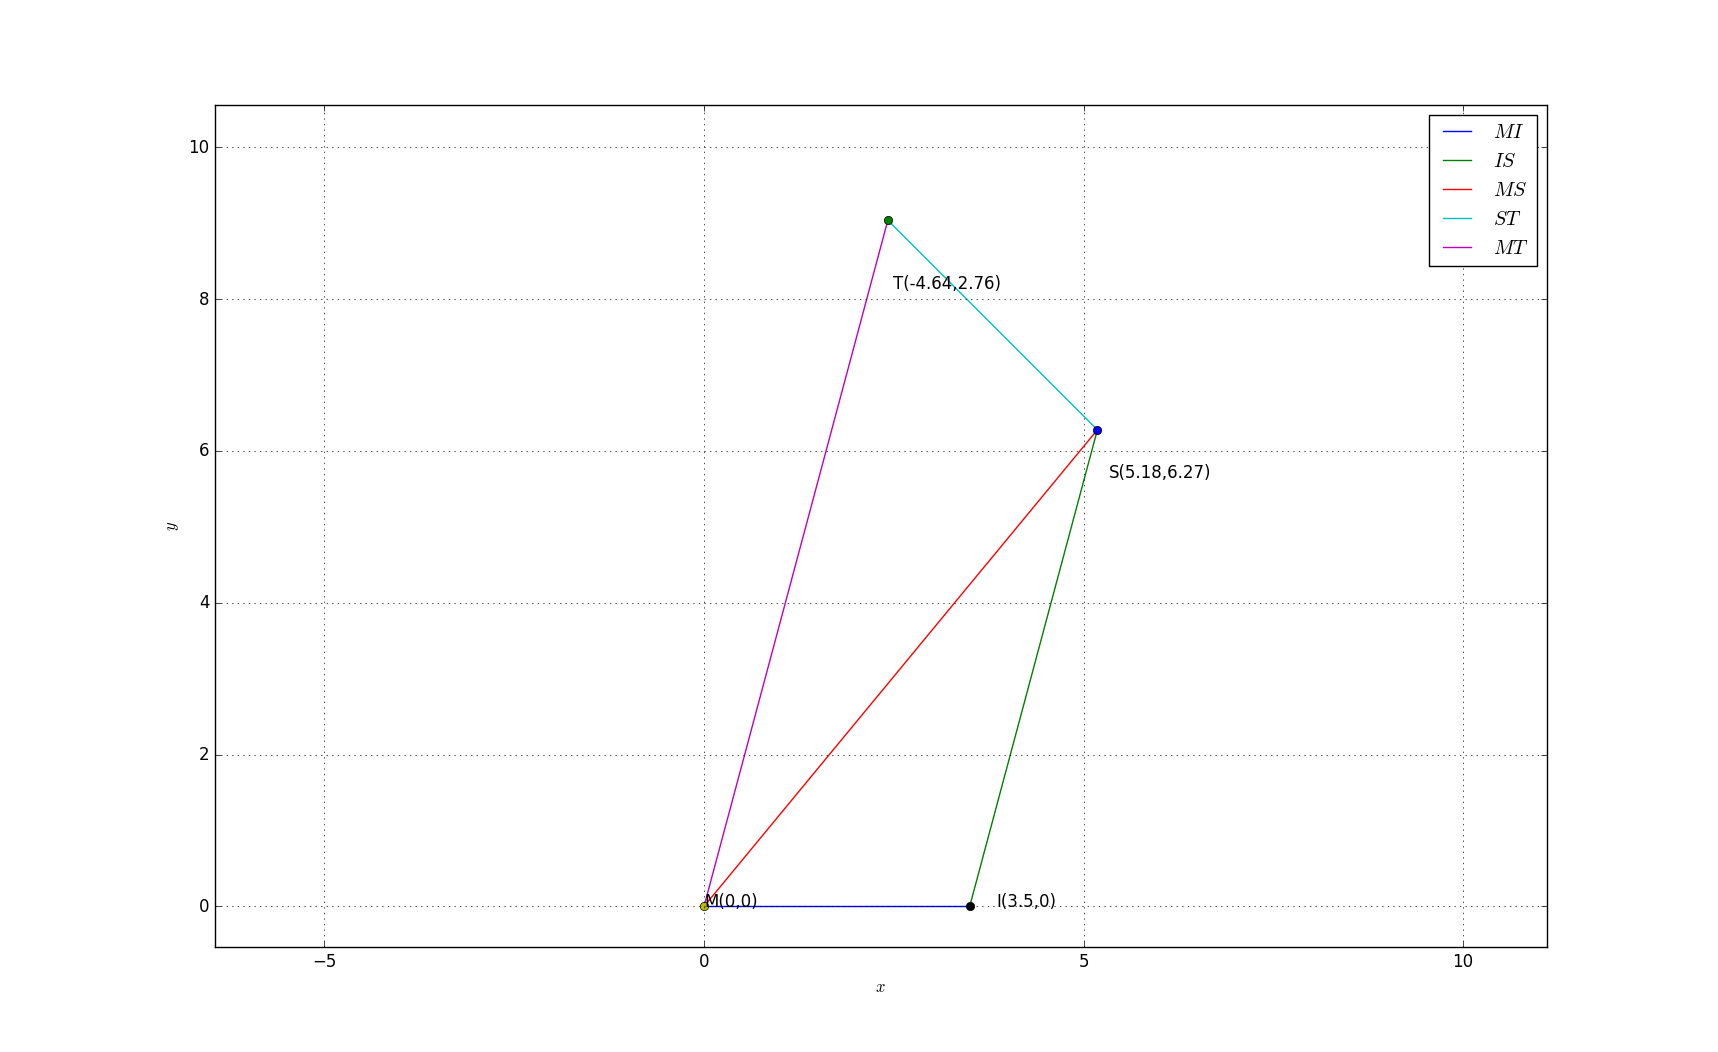
\includegraphics[scale=0.4]{./figs/quad/quad_constr1.png}
}
\caption{Quadrilateral with python}
\label{fig:foo}
\end{figure}
\begin{itemize}
\item \textbf{python :}\url{https://github.com/d-DP/geometryy/blob/master/codes/quad/quad_constr1.py}\\
\item \textbf{tikz:} \url{https://github.com/d-DP/geometryy/blob/master/figs/quad/quad_constr.tex}
\end{itemize}
\end{frame}
